\documentclass[a4paper,12pt]{article}
   % Packages and definitions:
   % {
      \usepackage{float}
      \usepackage[english]{babel}
      \usepackage[utf8]{inputenc}
      \usepackage{amsmath}
      \usepackage{amssymb}
      \usepackage{color}
      \usepackage{subcaption}
      \usepackage{booktabs}
      \usepackage{tikz}
      \usepackage{multirow}
      \usetikzlibrary{decorations.pathreplacing}
      \usepackage{graphicx,epstopdf}
      \usepackage{cleveref}
      \usepackage{collcell} % loads array
      \usepackage{listings}
      \usepackage{algorithm}
      \usepackage{algpseudocode}
      \newcolumntype{m}{>{$} r <{$}}
      \newcolumntype{u}{>{$[\collectcell\si} l <{\endcollectcell]$}}
      \newcommand{\approxtext}[1]{\ensuremath{\stackrel{\text{#1}}{=}}}
      \newcommand{\matr}[1]{\mathbf{#1}}
      \newcommand{\partt}[2]{\ensuremath{\dfrac{\d {#1}}{\partial {#2}}}}
      \renewcommand{\d}[1]{\ensuremath{\operatorname{d}\!{#1}}} % non-italized differentials
      \newcommand{\h}[0]{\ensuremath{\hbar}} % hbar
      \newcommand{\qed}[0]{\ensuremath{\tag*{$\square$}}} % QED square
      \def\changemargin#1#2{\list{}{\rightmargin#2\leftmargin#1}\item[]}
      \let\endchangemargin=\endlist 
      \usepackage{amsthm}
      \theoremstyle{plain}
      \newtheorem{thm}{theorem} % reset theorem numbering for each chapter
      \theoremstyle{definition}
      \newtheorem{defn}[thm]{definition} % definition numbers are dependent on theorem numbers
      \newtheorem{exmp}[thm]{example} % same for example numbers
      \bibliographystyle{natbib}
      \renewcommand{\theequation}{\thesection.\arabic{equation}}
      \newcommand{\ts}{\textsuperscript} 

      \definecolor{dkgreen}{rgb}{0,0.6,0}
      \definecolor{gray}{rgb}{0.5,0.5,0.5}
      \definecolor{mauve}{rgb}{0.58,0,0.82}

      \lstset{frame=tb,
        language=Java,
        aboveskip=3mm,
        belowskip=3mm,
        showstringspaces=false,
        columns=flexible,
        basicstyle={\small\ttfamily},
        numbers=none,
        numberstyle=\tiny\color{gray},
        keywordstyle=\color{blue},
        commentstyle=\color{dkgreen},
        stringstyle=\color{mauve},
        breaklines=true,
        breakatwhitespace=true,
        tabsize=3
      }
% }
\title
{
	\textbf
	{
      FYTN02: Computer simulation of the Ising model
   }
}

\author{Henrik Åhl\\}
\date{\today}

\begin{document}
\begin{titlepage}
	
   \maketitle 
	\begin{center}
		\phantom{a}
		{Department of Astronomy and Theoretical Physics, Lund University}
		\\[2cm]
		{Project supervised by Anders Irbäck}
		\vfill
		\includegraphics[height=4cm]{logocLUeng.pdf}
	\end{center}
	\thispagestyle{empty} % do not count pages just yet

\end{titlepage}

	\setcounter{equation}{0}
   \section{Problem 1}
    
   \paragraph{A}
      With H=0 and a 100x100 matrix, the critical temperature, defined as
      $T_c = 2.27$, indeed seems to be
      located around the theoretical exact value. The effect is however not
      instant, although the significant change seems to occur within the
      interval $T \in [T_c - 1, T_c+ 1]$.
   \paragraph{B}
      When instead the magnetization is studied, the rate of change can once
      again be seen to very gradual. It is on the other hand hard to here state
      an interval where the change is significant, due to the very apparent
      hysteresis reaction the model seems to exhibit. When starting out with a
      magnetization in either direction, the system tends to maintain that
      achieved state, so that in effect no change of state can be said to appear
      at a certain point in field-space. 
     
      It is apparent that the initial conditions of the system are largely a
      determining factor for how the magnetization develops under the influence
      of an external field. In effect, the only noticable consequence of gradual
      change within the $H$-range
      of $[-0.1, 0.1]$ seems to be that there is a small shift in the degree of
      magnetization. This might indicate that there is no significant phase
      shift when $T<T_c$.

    \section{Problem 2}

      One can in the latter exercise observe how small clusters tend to form in
      certain ways given different values on the magnetization. It is apparent
      that larger values support the forming of clusers with increasing sizes.
      However, with a random initial configuration it is hard to draw any
      adequate conclusions from the attained output of the model; larger 
      clusters seems to appear as the magnetization
      increases, but not in any clear, determinable way. It could be reasoned
      that with a larger magnetization, the coupling terms in the energy
      function become big enough to counteract the tendency to align according
      to the magnetization. 

      When comparing to when the overall initial state is not randomly
      configured, but instead takes a circular shape, clusters are not as likely
      to form, which ought to be because of the rigidness that comes with an
      initial, stable configuration -- when the spins are already aligned
      according to their neighbours, they become unwilling to change. 
      However, some boundary effects are nevertheless present, as is to be
      expected according to the looks of the energy function, as the boundary
      essentially constructs a probabilistic fringe-zone. 
   

      \begin{figure}[H]
         \centering
          \begin{subfigure}[t]{0.3\textwidth}
            
\includegraphics[width=\textwidth]{398.png}
              \caption*{$M=-0.98$}
          \end{subfigure}
          ~
          \begin{subfigure}[t]{0.3\textwidth}
            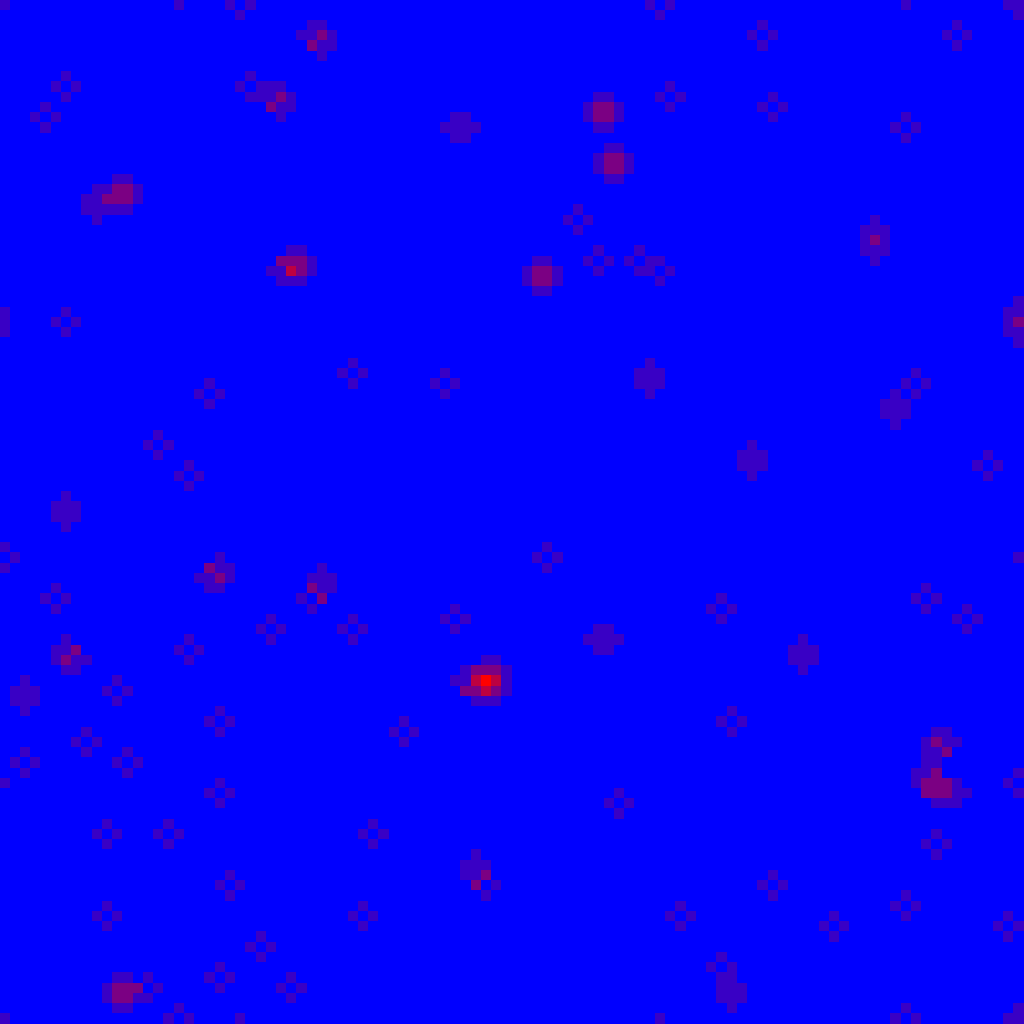
\includegraphics[width=\textwidth]{397.png}
              \caption*{$M=-0.97$}
          \end{subfigure}
          ~
          \begin{subfigure}[t]{0.3\textwidth}
            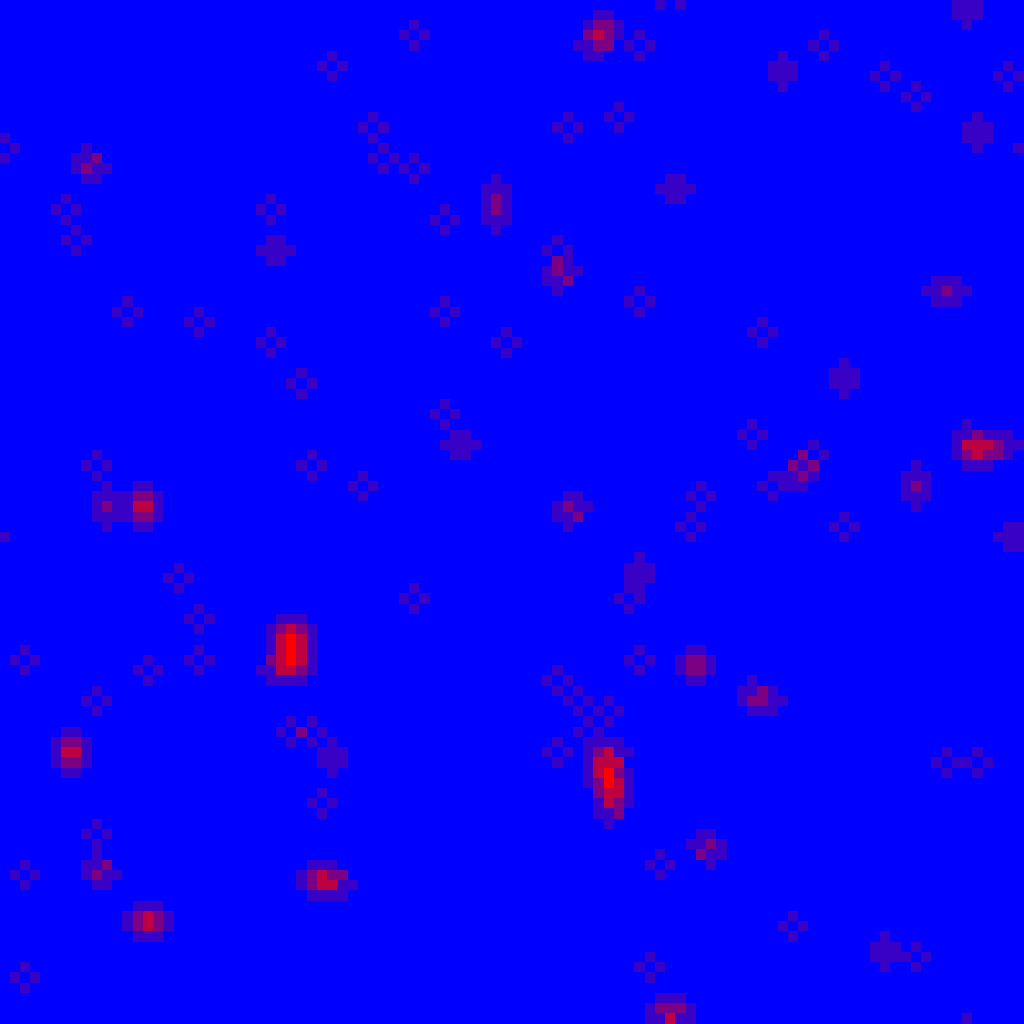
\includegraphics[width=\textwidth]{396.png}
             \caption*{$M=-0.96$}
          \end{subfigure}
          \caption*{Random initial configuration}
      \end{figure}

      \begin{figure}[H]
         \centering
          \begin{subfigure}[t]{0.3\textwidth}
            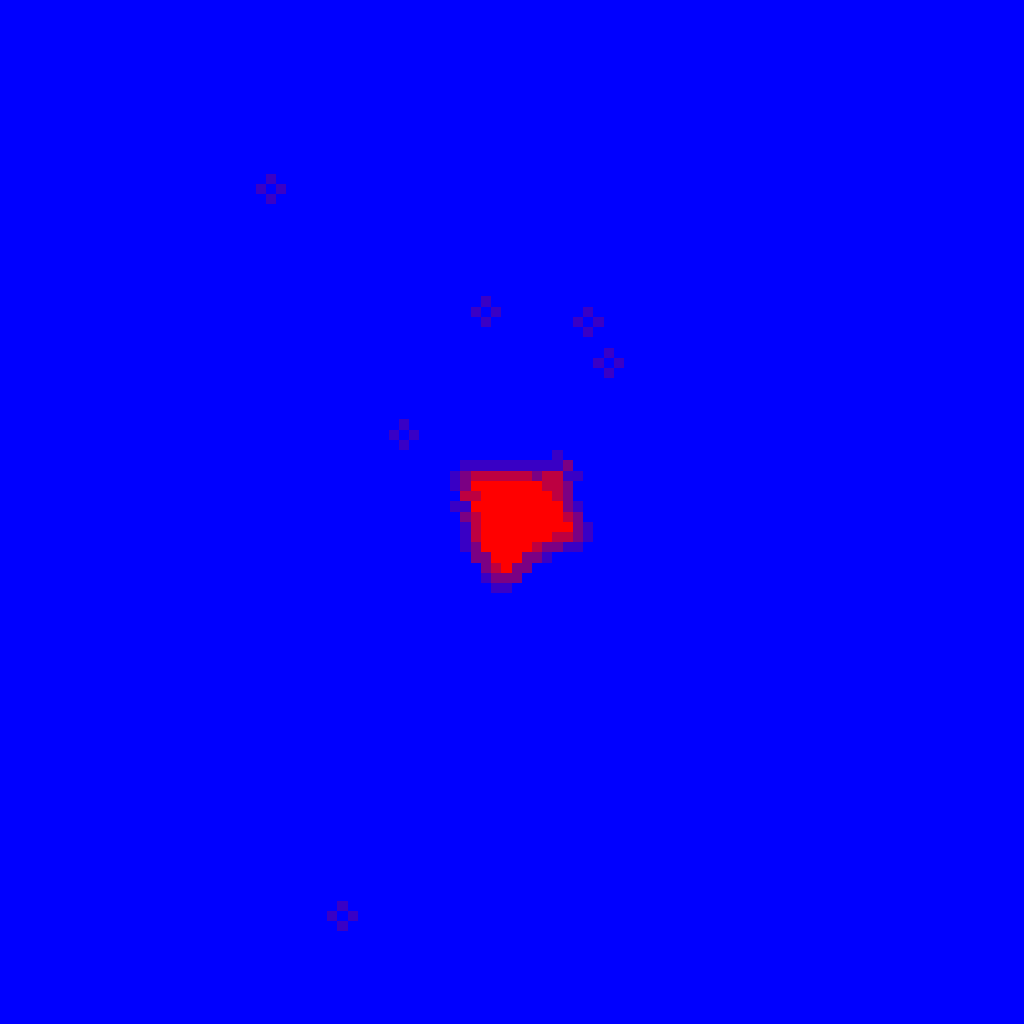
\includegraphics[width=\textwidth]{398c.png}
              \caption*{$-M=-0.98$}
          \end{subfigure}
          ~
          \begin{subfigure}[t]{0.3\textwidth}
            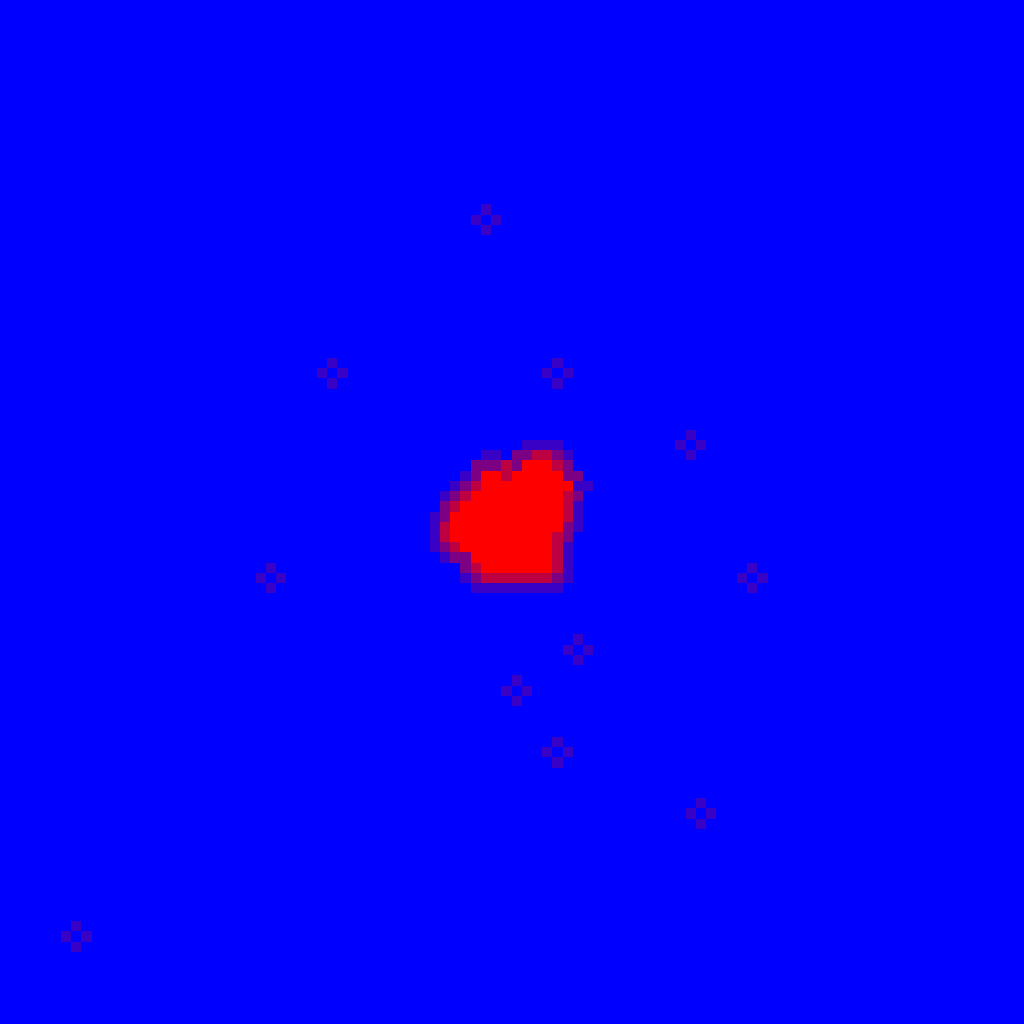
\includegraphics[width=\textwidth]{397c.png}
              \caption*{$M=-0.97$}
          \end{subfigure}
          ~
          \begin{subfigure}[t]{0.3\textwidth}
            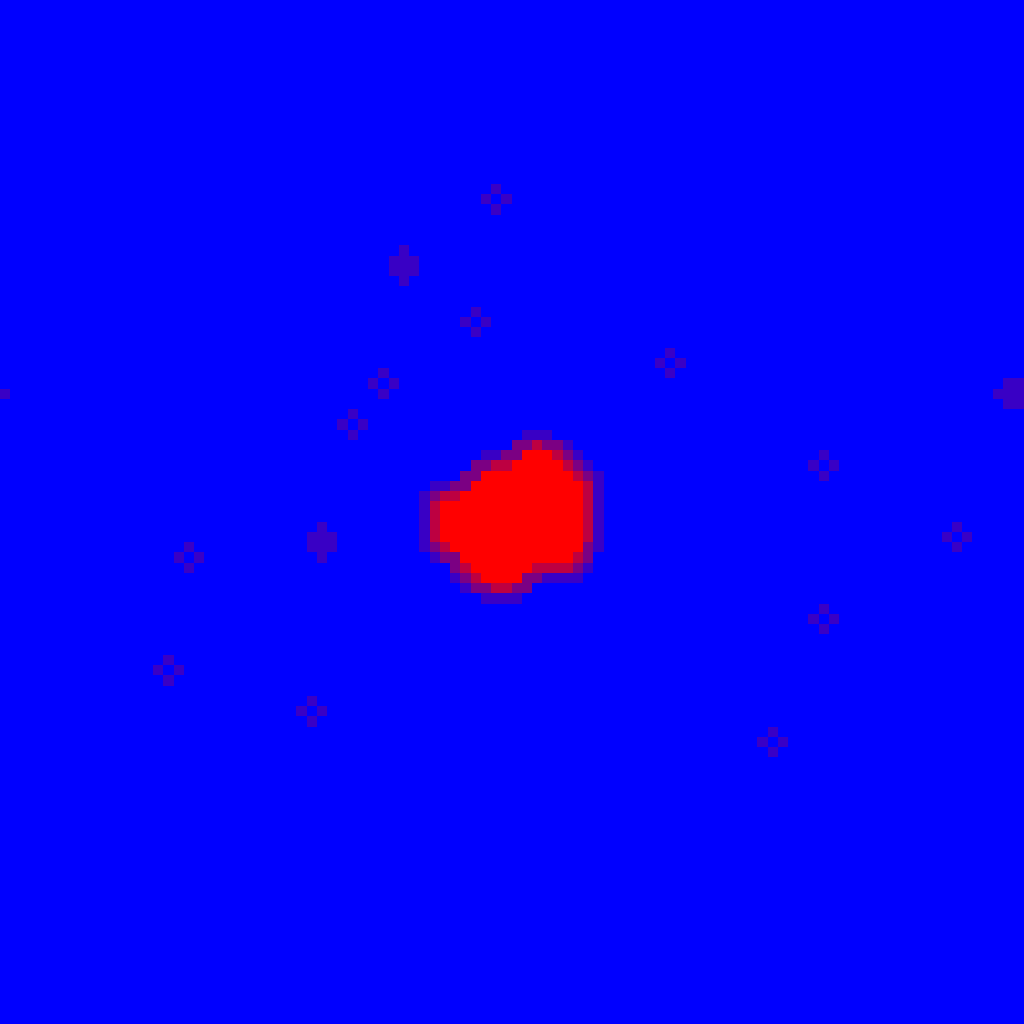
\includegraphics[width=\textwidth]{396c.png}
             \caption*{$M=-0.96$}
          \end{subfigure}
          \caption*{Circular initial configuration}
      \end{figure}
            
\end{document}

